\section{Análisis e introducción a las técnicas de SLAM}
El SLAM\textit{(Simultaneous Localization and Mapping)} es una técnica cuyo objetivo es contruir un mapa de un entorno desconocido con un robot móvil 
y conocer la posición de dicho robot dentro del mapa. \\
El primer planteamiento de la resolución de estos dos problemas cómo son la localización de un robot y la creación de mapas de manera conjunta surgió 
en 1986 en un congreso del IEEE en San Francisco. \\
Durante aquellos años, se había comenzado a introducir métodos probabilístico en la inteligencia artificial 
y en la robótica. En dicha conferencia, se llegó a la conclusión de que la generación de mapas consistentes y la localización de manera probabilistica era
un problema fundamental.\\

Tras ello, se establecieron las bases estadisticas para describir la relaciones entre \textit{landmarks}, objetos de referencia y 
para manipular la incertidumbre geométrica. \\
El planteamiento básico del problema de SLAM es el mostrado a continuación:
\begin{figure}[h!]
    \centering
    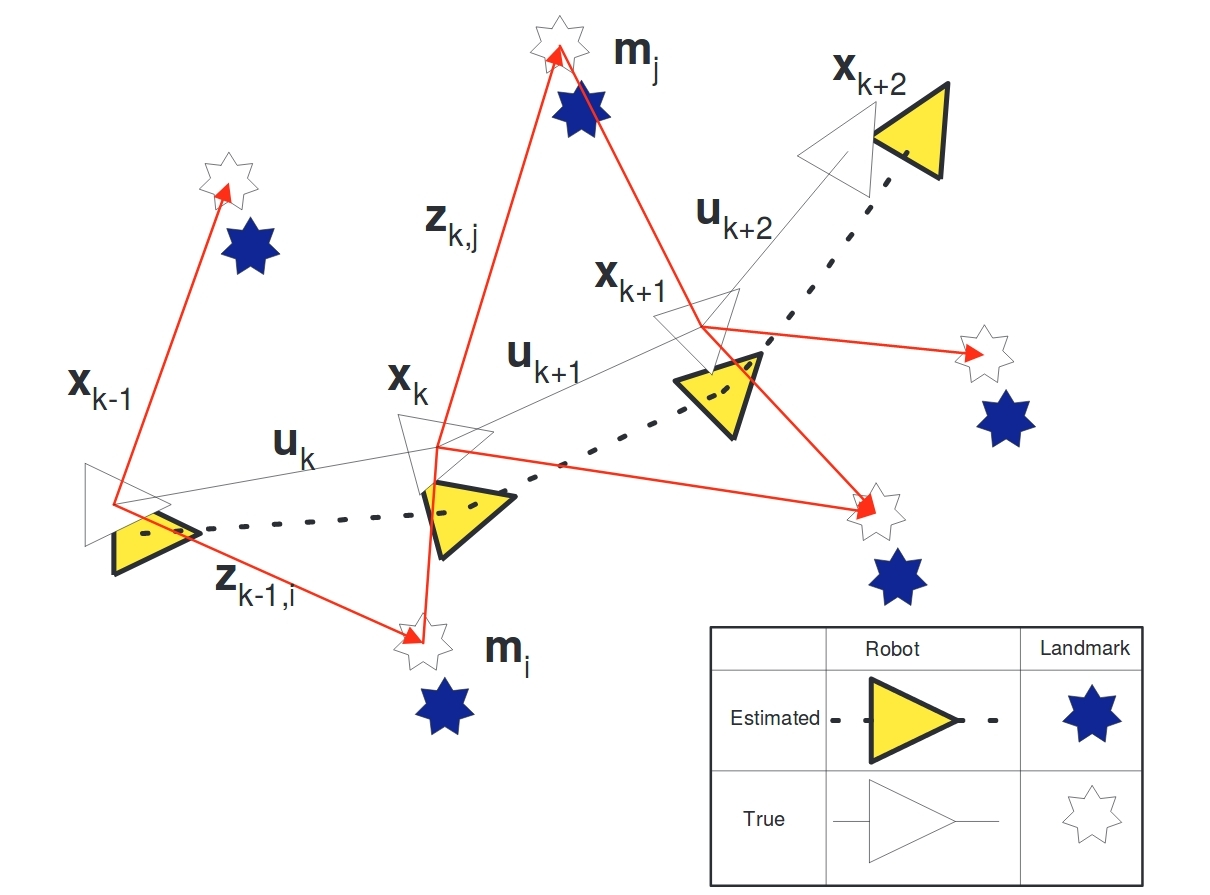
\includegraphics[width=.6\textwidth]{images/slam_prob}
    \caption{Problema básico de SLAM}
\end{figure}

Dado un robot que se mueve por un entorno desconocido, tomando observaciones relativas de un número desconocido de landmarks empleando un sensor posicionado
en el robot; para el instante \textit{k}, se definen las siguientes variables:
\begin{itemize}
    \item $\textbf{x}_k$: Vector de estados que describe la posición y orientación del vehículo.
    \item $\textbf{u}_k$: Vector de control aplicado el instante anterior sobre el vehículo para que se encuentre
en el estado $\textit{x}_k$ en el instante \textit{k}.
    \item $\textbf{m}_i$:Vector que describe la posición del i-ésimo landmark cuya verdadera ubicación se supone invariable con el tiempo.
    \item $\textbf{z}_{ik}$: Observación tomada desde el vehiculo de la posición del i-ésimo landmark en el instante \textit{k}.
\end{itemize}
Por tanto, se deberá computar la siguiente distribución probabilística en cada instante \textit{k}:
\begin{equation}
    P\Big( \textbf{x}_k ,m | \textbf{Z}_{0:k},\textbf{U}_{0:k},x_0\Big)
\end{equation}
La solución se obtendrá de manera recursiva empleando el teorema de Bayes en un proceso en dos pasos: \textit{Time-Update} y \textit{Measurement-Update}. Para ello,
será necesario conocer el modelo de observación y el de movimiento. \\

\begin{center}
    $P\Big( \textbf{z}_k | \textbf{x}_{k},m \Big)$ \hspace{2cm} $P\Big( \textbf{x}_k | \textbf{x}_{k-1},\textbf{u}_{k} \Big)$
\end{center}

Una vez planteado de manera superficial el problema a resolver, el modo de abordarlo se ha desarrollado en muchas direcciones durante los últimos 20 años. \\
Algunos de estos métodos se muestran a continuación y se hablará de ellos, para posteriormente indagar en dos técnicas concretas.
\subsection{Clasificación técnicas de SLAM}
La forma en que se toma información de las imágenes que recibe y de su entorno y cómo la procesa permite distinguir los siguientes tipos de sistemas
SLAM visual:
\begin{itemize}
\item \textit{Denso vs Disperso} \\
En función de la cantidad de datos tomada de cada imagen, se realizará ésta clasificación. Las técnicas de SLAM disperso sólo emplean una pequeña
región de píxeles, cómo pueden ser puntos característicos. \\
Sin embargo, las técnicas densas emplean la mayoría o todos los píxeles de cada frame que reciben. \\

Debido a que la cantidad y tipo de información que toman son diferentes, el tipo de mapa que se obtendrá también lo es. Con las técnicas de SLAM
disperso se obtendrá una nube de puntos que será una representación de los puntos característicos de las escena y se usará sobre todo para hacer
un tracking de la pose de la cámara. Por otro lado, un mapa denso tendrá muchos más detalles y, requerirá una carga computacional más elevada.

 \item \textit{Directo vs Indirecto} \\
En función de cómo las técnicas de SLAM empleen y traten la información que reciben, se podrá clasificar en SLAM directo o indirecto.\\
El SLAM Indirecto, se basa en extraer primero las features de la imagen, puntos característicos, para posteriormente emplearlos para localizarse y contruir
el mapa. Para extraer estos puntos característicos existen muchos descriptores: ORB, SIFT, FAST, etc. \\

En contraste, el SLAM Directo, emplea directamente la intensidad de los píxeles, de tal modo que se obtengan features intermedios. Estos métodos tratan de 
obtener la profundidad y estructura del entorno a partir de una optimización del mapa. Los procesos de extracción de puntos característicos son mucho más
pesados computacionalmente si se trabaja al mismo rate que un slam indirecto.\\
Por último, destacar, que los métodos indirectos de SLAM son más tolerántes a los cambios de iluminación del entorno.\\

A continuación, se mostrará una comparativa de una serie de técnicas de SLAM:
\begin{figure}[h!]
    \centering
    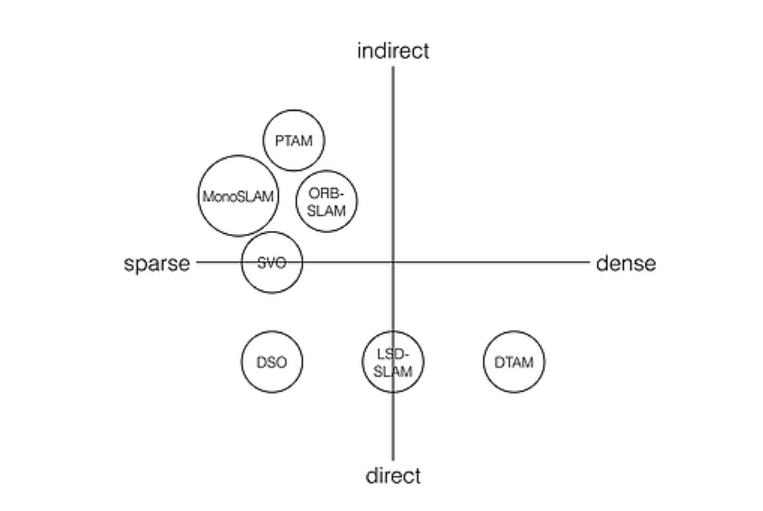
\includegraphics[width=.6\textwidth]{images/comp_slam}
    \caption{Comparativa de técnicas SLAM}
\end{figure}

\end{itemize}

\subsection{Técnicas SLAM implementadas en éste proyecto}
Destacar que, mientras la primera metodología de SLAM es una técnica determinista, la segunda será probabilistica.
\subsubsection{\textit{RTAB-Map SLAM}}
RTAB-Map \textit{(Real-Time Appearance-Based Mapping)} es una técnica de Graph-SLAM \footnote{http://robots.stanford.edu/papers/thrun.graphslam.pdf} basada en la detección de bucles cerrados incrementales. Es totalmente funcional 
con sensores RGB-D, Stereo y LIDAR. \\
El detector de bucles cerrados se basará en la comparativa de cuán semenjantes son la imágenes en una localización y la previa. Cuándo una hipótesis 
de bucle cerrado es aceptada, se añade una nueva restricción al \textit{graph} del mapa y, tras ello, el optimizador minimiza el error del mapa. \\

\begin{figure}[h!]
    \centering
    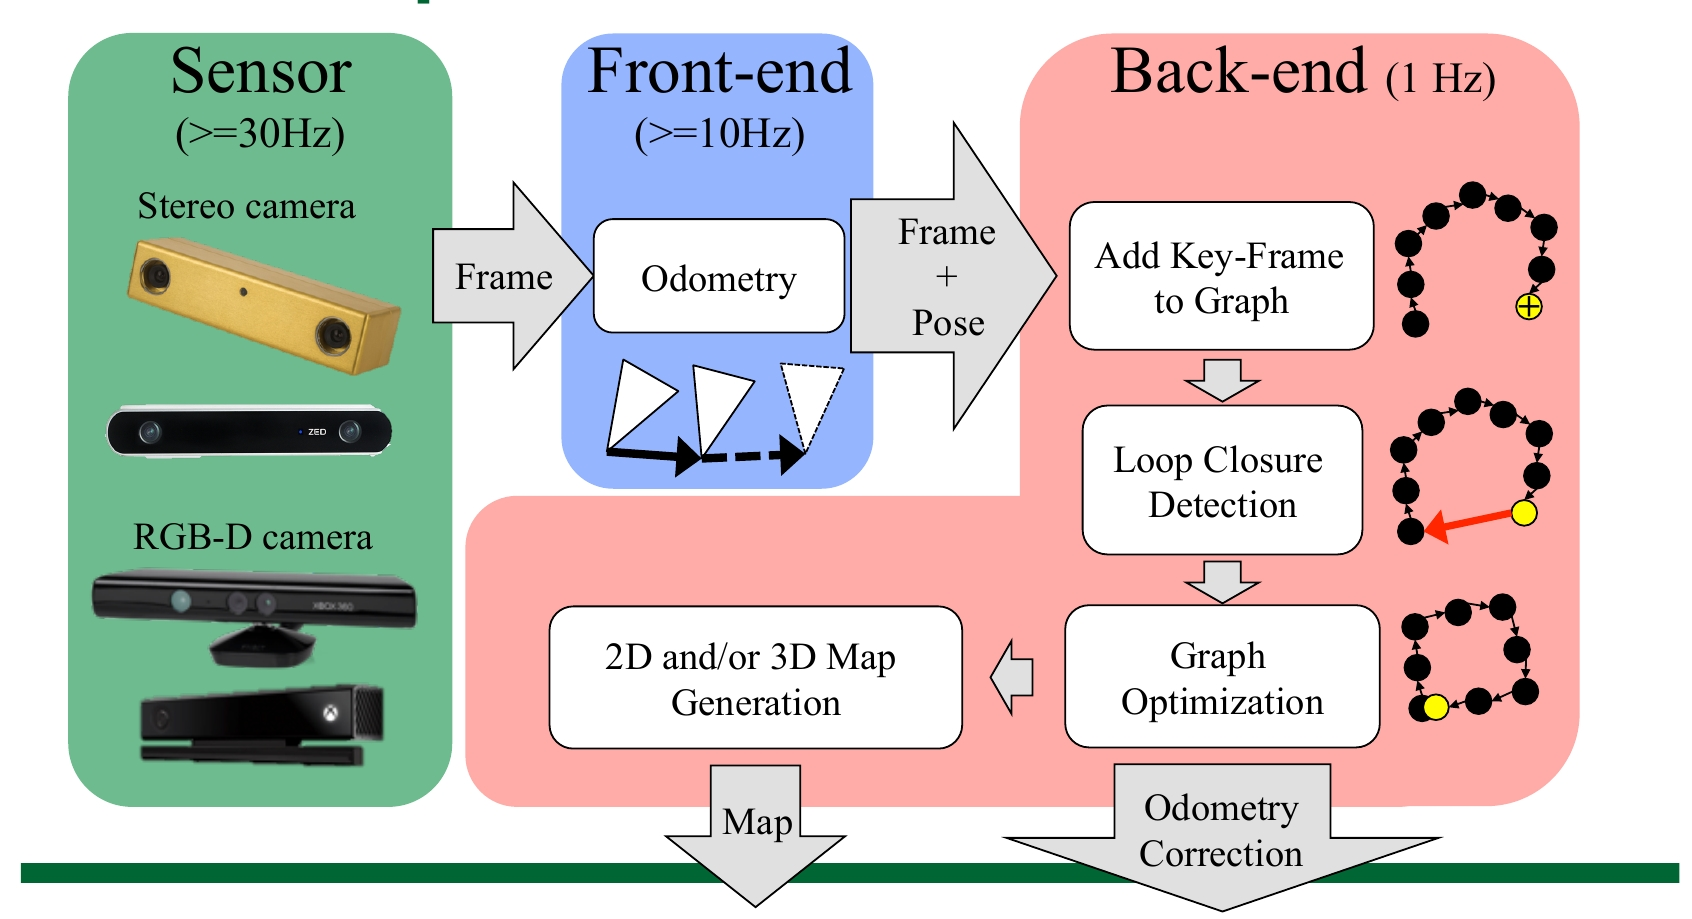
\includegraphics[width=.7\textwidth]{images/rtabmap_scheme}
    \caption{Esquema del Back-End y Front-End de RTAB-Map}
\end{figure}


Este algoritmo plantea una estrategia de particionado de memoria que pretende asemejarse al funcionamiento de la memoria humana, 
dónde ésta se estructura en: \\
Memoria de trabajo del robot \textit{(Working Memory)}, memoria a largo plazo \textit{(Long Term Memory)}, 
memoria a corto plazo \textit{(Short-term memory)} y memoria sensorial \textit{(Sensory Memory)}. \\
De ese modo, se mantendrán en la memoria de trabajo del robot aquellas localizaciones que se han visitado recientemente 
y con más frecuencia, mientras que el resto pasarán a la memoria de largo plazo. \\

\begin{figure}[h!]
    \centering
    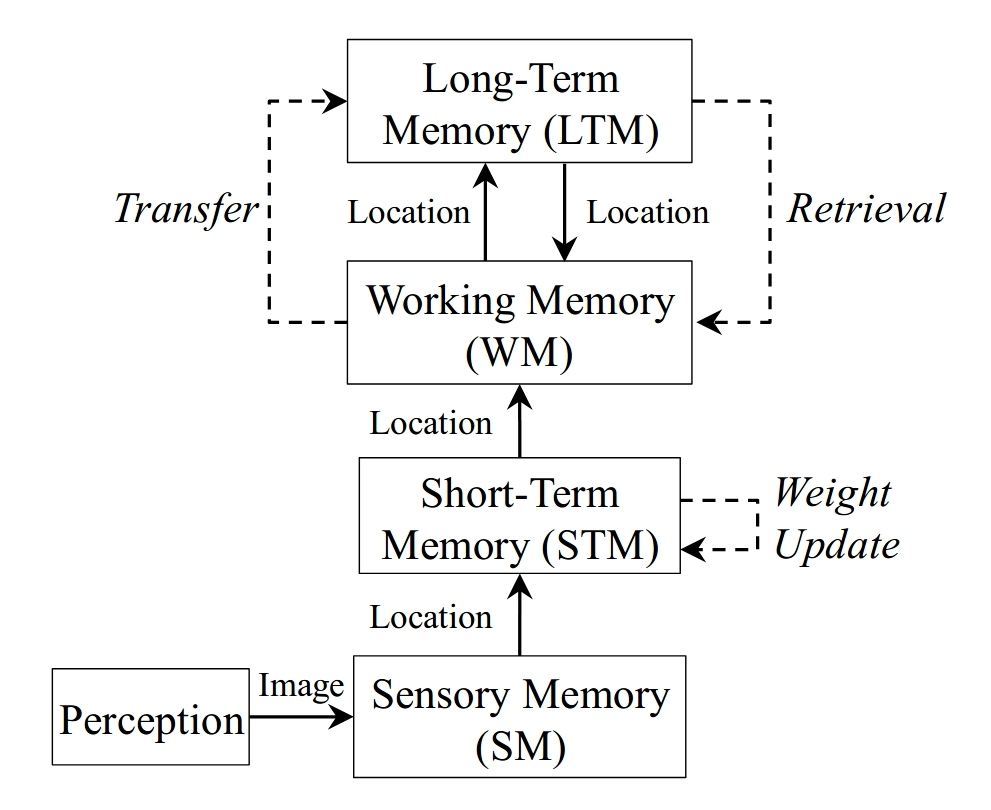
\includegraphics[width=.4\textwidth]{images/rtabmap_memory}
    \caption{Estructura de memoria de la técnica RTAB-Map}
\end{figure}


Se partirá de la premisa de que aquellas localizaciones que son visitadas de forma más frecuente son más propensas a 
crear bucles cerrados. Por ello, el número de veces que una localización sea visitada será empleado cómo peso, de 
esta forma serán transferidas desde la memoria de trabajo a la memoria de largo plazo aquellas observaciones que 
tengan mayor peso.\\
La memoria a corto plazo, \textit{STM}, tiene cómo misión buscar las similitudes que existan entre dos imágenes
consecutivas, mientras que la memoria de trabajo, \textit{WM}, es la encargada de detectar los bucles cerrados entre las
localizaciones en el espacio. El número de localizaciones almacenadas en la memoria del trabajo del robot es
limitado. El tamaño de la memoria a corto plazo, \textit{STM}, está basado en la velocidad del robot y en la frecuencia de
adquisición de las localizaciones. \\

% NO SE SI METER ESTA PARTE
\begin{comment}
Es importante destacar que todas las observaciones almacenadas en la memoria a largo plazo, \textit{STM}, del robot no se
usan para detectar bucles cerrados. No obstante, es importante elegir cuidadosamente las localizaciones que se
almacenan en esta memoria. Almacenar las observaciones según la técnica FIFO (First In First Out), sería un
error debido a que, cómo el algoritmo establece un número máximo de localizaciones que se pueden
almacenar mientras se está explorando un entorno, podríamos alcanzar el superar el umbral de tiempo
establecido sin llegar a cerrar el bucle haciendo que las localizaciones más antiguas nunca consigan asociarse. \\
cómo alternativa, el orden de almacenamiento de las observaciones se elige de forma aleatoria, aunque es
preferible mantener en la memoria de trabajo aquellas localizaciones que son más susceptibles de ser
observadas.
\end{comment}
\subsection{Framework de optimización Octomap}
El paquete de ROS empleado para emplear la ténica RTAB-Map,\textit{rtabmap-ros}, posee la posibilidad de extraer también el mapa de ocupación 2D y 3D gracias al Framework 
\textit{Octomap}\footnote{https://octomap.github.io/}. \\
Este framework es una librería de C++ que permite la obtención de mapas probabilísticos basándose en una estructura de representación jerárquica de datos para subdividir
el espacio 3D, esta estructura es denominada \textit{Octotrees}. \\

\begin{figure}[h!]
    \centering
    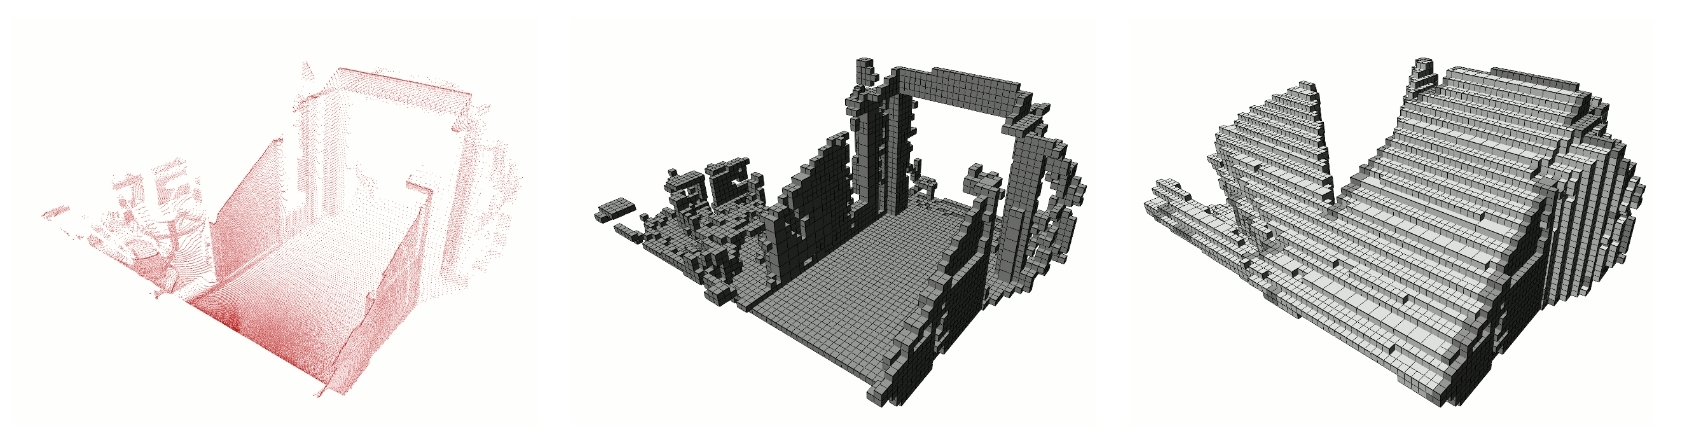
\includegraphics[width=.9\textwidth]{images/octomap_beauty}
    \caption{Optimización realizará empleando los \textit{Octotrees}}
\end{figure}


Los \textit{Octotrees} se emplean para almacenar propiedades booleanas del entorno, en el caso de
la robótica estas propiedas booleanas es la ocupación de dicha celda, de la cual es posible definir su tamaño mínimo en función de la resolución de mapa
deseada.
\begin{figure}[h!]
    \centering
    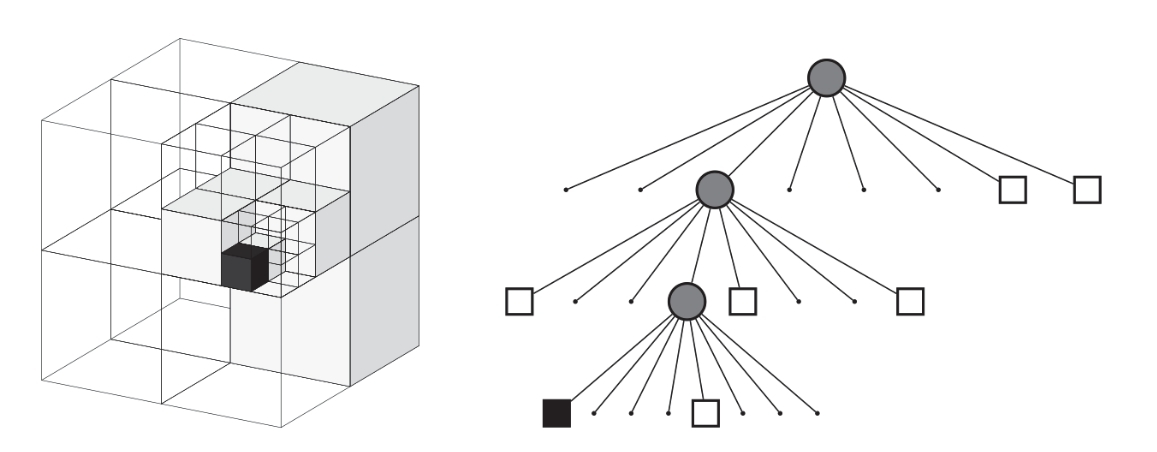
\includegraphics[width=.7\textwidth]{images/octotree}
    \caption{Funcionamiento del \textit{octotree} y su estructura en árbol}
\end{figure}

\newpage
\subsubsection{\textit{ORB-SLAM 2}}
ORB-SLAM2 es una técnica de SLAM en tiempo real para cámaras Monocular, Stereo y RGB-D que se engloba dentro de las técnicas de 
\textit{Sparse-Slam}. Se computa la trayectoria y hace una reconstrucción dispersa 3D del entorno. Al igual que todas las técnicas 
de SLAM, se basa en la detección de bucles cerrados y  se relocaliza en tiempo real. \\
Se basa en la detección de \textit{keyframes} que emplea para hacer un tracking de los mismos y a partir de ello crear el 
mapa local que, posteriormente, se optimizará junto al mapa global. \\
Unos de los puntos destacables de ésta técnica de SLAM son los siguientes:
\begin{itemize}
    \item Emplea \textit{grafo de covisibilidad}. Tanto el seguimiento cómo el mapping se focalizan en el área covisible,
    independientemente del tamaño del mapa completo, consiguiendo así explorar entornos amplios sin
    aumentar el tiempo y la carga de computación.

    \item La estrategia para detectar los bucles cerrados de visión en tiempo real se basa en la optimización de
   un de grafo denominado \textit{Essencial Graph}, lo cuál se desarrollará mas adelante.
\end{itemize}

A continuación, se tratará un poco el funcionamiento interno del algoritmo, el cuál presenta el siguiente esquema:
\begin{figure}[h!]
    \centering
    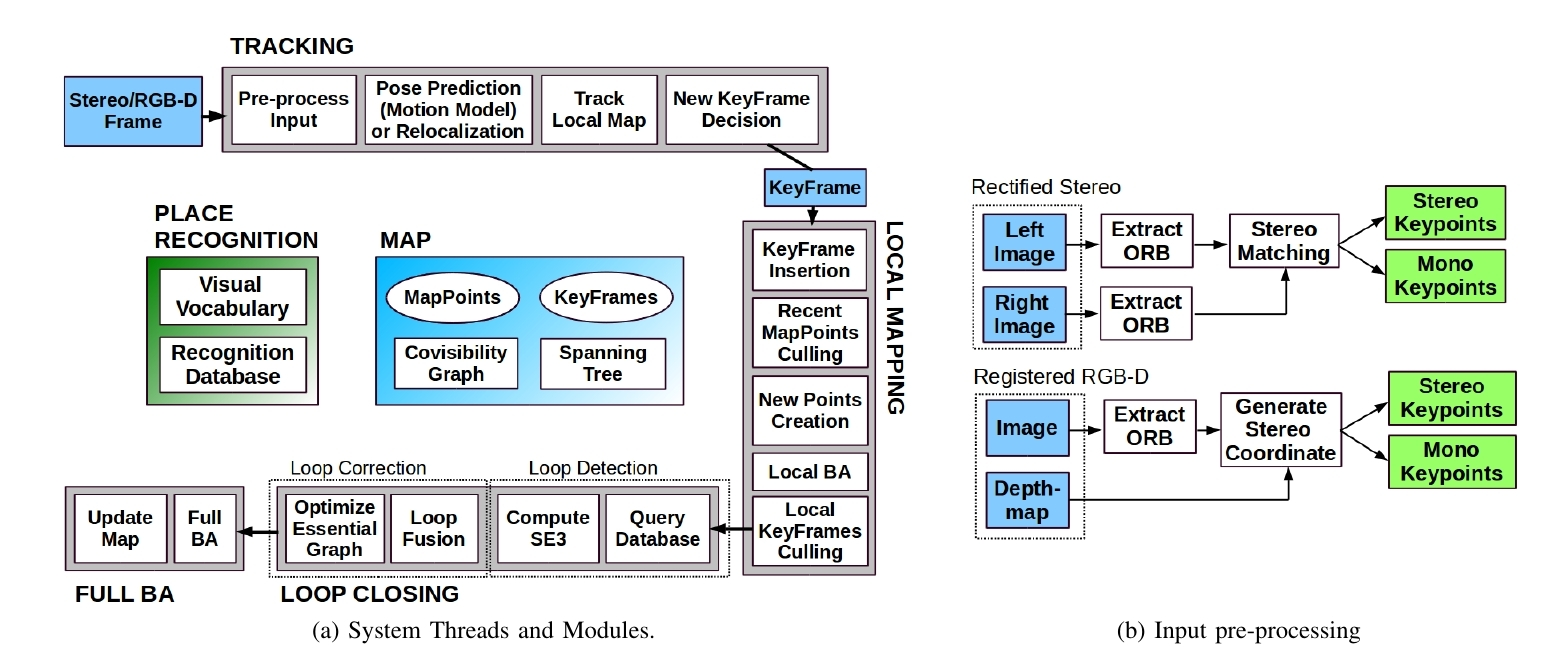
\includegraphics[width=1\textwidth]{images/orb_scheme}
    \caption{Estructura interna de ORB-SLAM2}
\end{figure}

Se observa cómo existen 6 grandes módulos, los cuales de lanzarán en 3 hilos paralelos. \\
En primer lugar, se tendrá el preprocesamiento de la imagen, de la cuál se obtendrán  ORB features 
\textit{(Oriented Fast and Rotated BRIEF)}. \\
Los hilos desempeñarán las siguientes funciones:
\begin{itemize}
    \item El \textit{tracking} se encargará de localizar la cámara en cada frame buscando marches entre las features
    del mapa local y minimizando la reprojección del error aplicando un \textit{Bundle Adjustment}\footnote{https://homes.cs.washington.edu/~sagarwal/bal.pdf} sólo de 
    movimiento.
    \item El \textit{Local Mapping} se encargará de gestionar y optimizar el mapa local aplicando un \textit{BA} local.
    \item El hilo de \textit{Loop Closing} se encargará de detectar bucles cerrados grandes y corregir la deriva acumulada
    realizando una optimización del grafo del \textit{pose} obtenido. Este hilo, lanza 4 hilos internos que se encagarán de
    realizar un \textit{Bundle Adjustement} completo tras la optimización del grafo del \textit{pose}, para hayar la solución
    más optima.
\end{itemize}

En caso de que el sistema pierda el tracking, lleva integrado un modulo de \textit{Plane recognition} basado en un vocabulario 
de palabras que básicamente funciona cómo un preentrenamiento de la técnica, para poder obtener y asociar keyframes más fácilmente. \\

En la imagen a continuación, puede observarse la técnica corriendo en un ordenador. Destacar que ésta técnica de SLAM presenta una carga computacional bastante elevada.
\begin{figure}[h!]
    \centering
    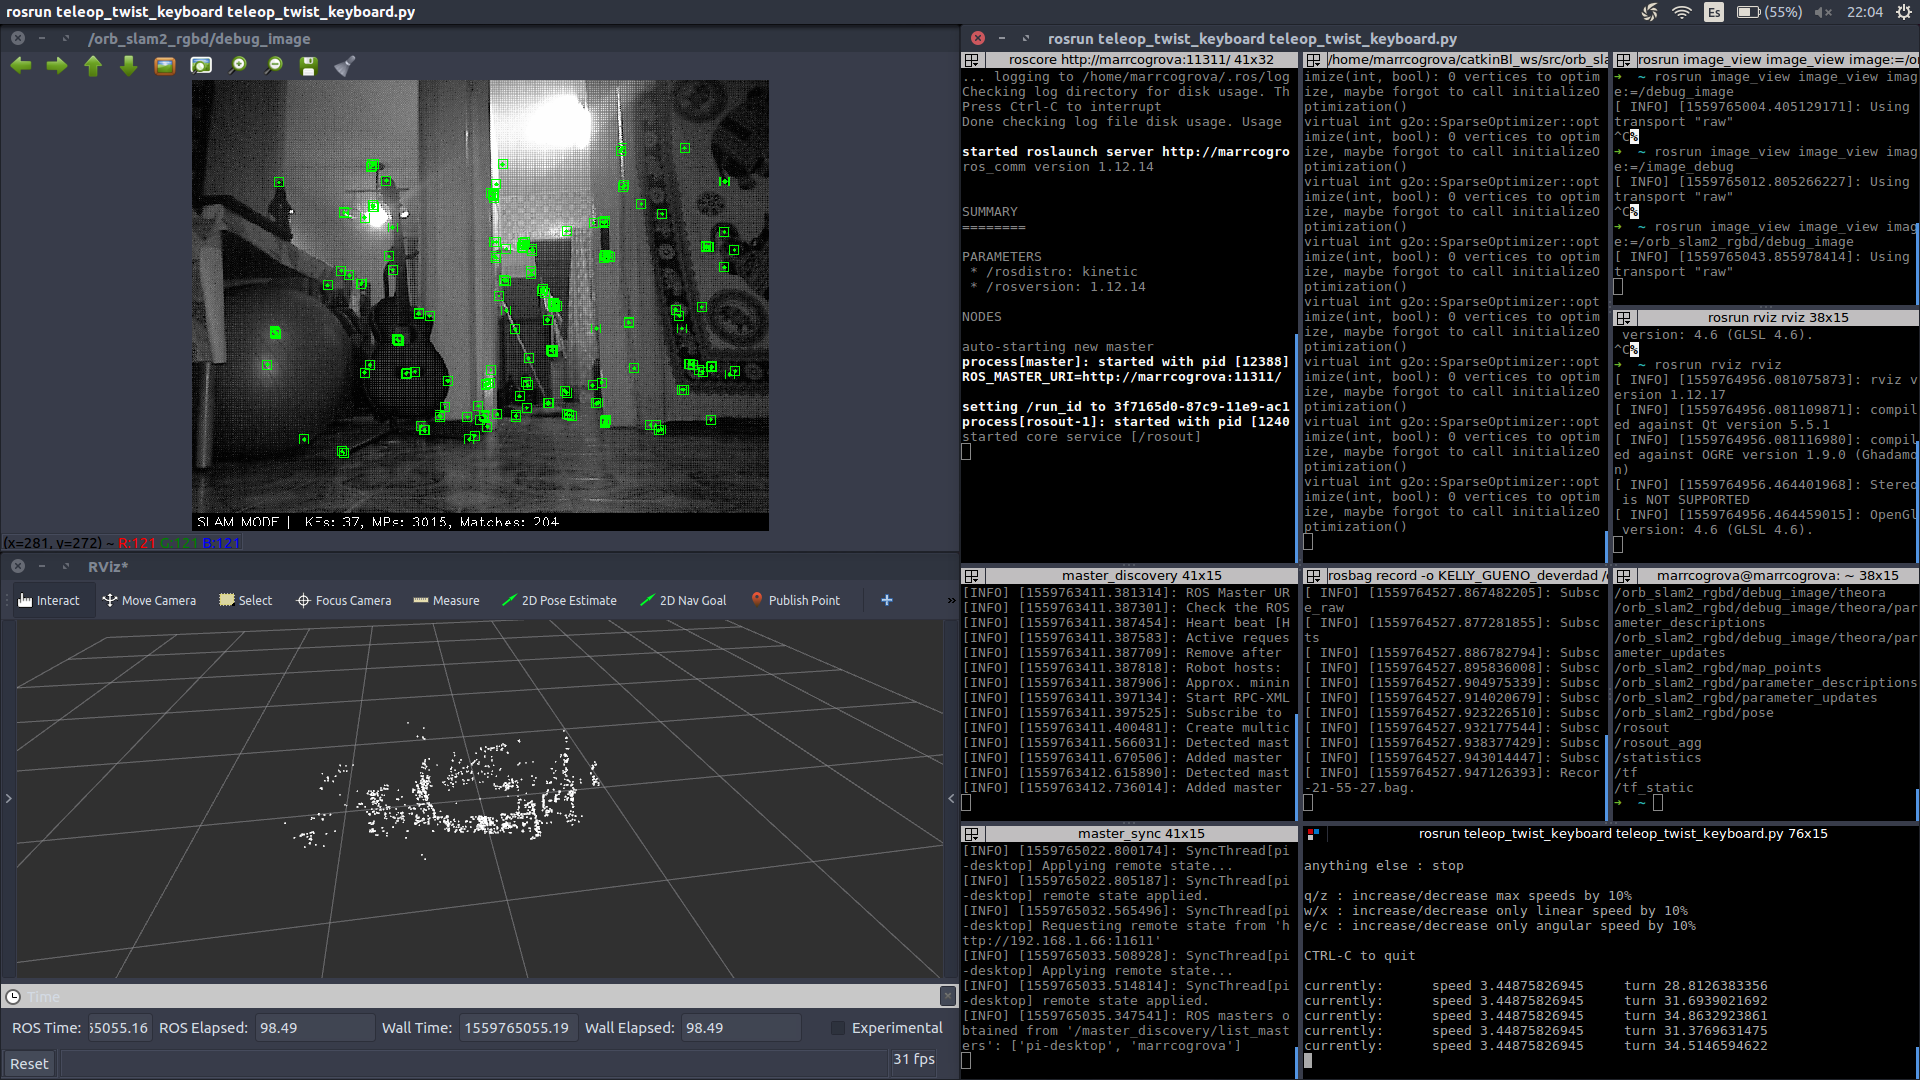
\includegraphics[width=1\textwidth]{images/working_zone_orb}
    \caption{ORB-SLAM2 en funcionamiento}
\end{figure}

Se observa en la imagen superior izquierda las features que está obteniendo en ese frame, a partir de las cuales se ha creado el mapa local y,
por extensión el global. En la imagen inferior izquierda, se puede observar el mapa creado, el cuál se analizará más tarde.\\
Por último, a la derecha se tienen las terminales a partir de las cuales se ha lanzado el SLAM y se realiza la comunicación con el robot.\\

\newpage

\section{Comparativa de resultados empleando \textit{rosbags} del robot}
Para realizar un análisis y una comparativa entre éstas dos técnicas de SLAM, se ha optado por generar un set de datos del robot y correrlo con ambas técnicas,
de tal modo que ambas téngan los mismos datos de entrada y se pueda analizar de mejor modo la salida de la arquitectura. \\
Aunque normalmente se correría el robot junto con el SLAM, si no se hubieran grabado estos set de datos sería más complejo comparar éstas técnicas. \\
Estos datasets, que han sido grabados en forma de \textit{rosbag}, se grabaron desde el ordenador en el que corre el SLAM, de todos los topicos que se recibian
del ordenador de abordo del robot a través de la comunicación \textit{Multi-master} implementada.\\
A continuación, se muestra una imagen de los topicos contenidos en ambos datasets:
\begin{figure}[h!]
    \centering
    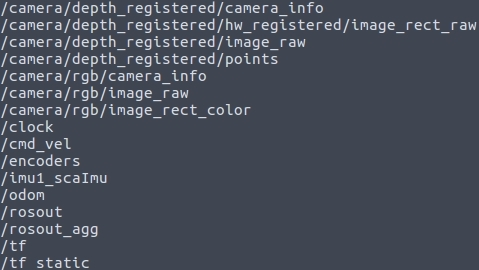
\includegraphics[width=.5\textwidth]{images/topics_bags}
    \caption{topicos contenidos en el bag}
\end{figure}

En ambos datasets el robot recorrerá un camino en torno al salón de la casa de uno de los integrantes del grupo. En el primer dataset, el estado del salón será 
el comun, de modo que haya una parte del mapa que no contendrán muchas features. Sin embargo, en el segundo se colocaron objetos en zonas dónde la cantidad de features
y los contrastes del mapa eran reducidos para así comparar el resultado inicial con uno en un entorno experimental, dónde se ha forzado que el entorno esté lleno de features.\\

Se realizarán 3 pruebas, las cuales se encuentras recogidas en vídeos existentes en la carpeta del proyecto. En primer lugar se mostrará el mapa creado por \textit{RTAB-Map} y
la estimación del \textit{path} del robot. Tras ello, se mostrará el mapa de ocupación generado por \textit{OctoMap} tanto en 2D cómo en 3D y, por último, se mostrará el
resultado obtenido con \textit{ORB-SLAM2 RGB-D}. \\

Destacar que, se pueden observar los resultados de las técnicas de SLAM en el directorio \textit{videos\_wheeleSLAM} de éste proyecto.
\newpage

\subsection{Análisis de resultados con el primer \textit{rosbag}}
Este dataset será el que contendrá el salón en un estado comun, sin alterar la cantidad de features existentes en el entorno. \\
En él, se recorrerá un camino de, aproximadamente, 1$m^2$ en torno al salón.

\subsubsection{RTAB-Map y local path}
En primer lugar, se mostrará el mapa denso obtenido gracias a RTABMAP. Se observa cómo el loop closure del mapa ha funcionado correctamente, de tal modo que la estructura final
del mapa será el rectangulo que confirma el salón.
\begin{figure}[h!]
    \centering
    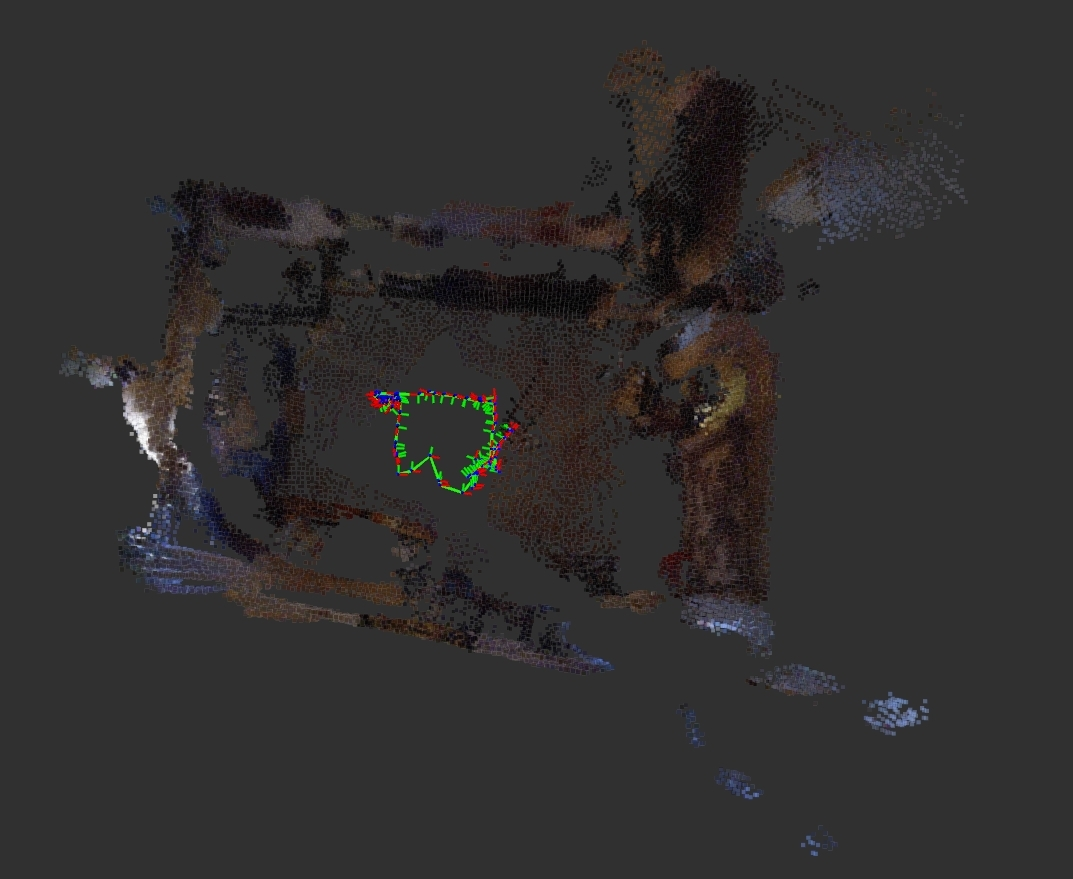
\includegraphics[width=.4\textwidth]{images/slam/bag1_rtabmap_noLC}
    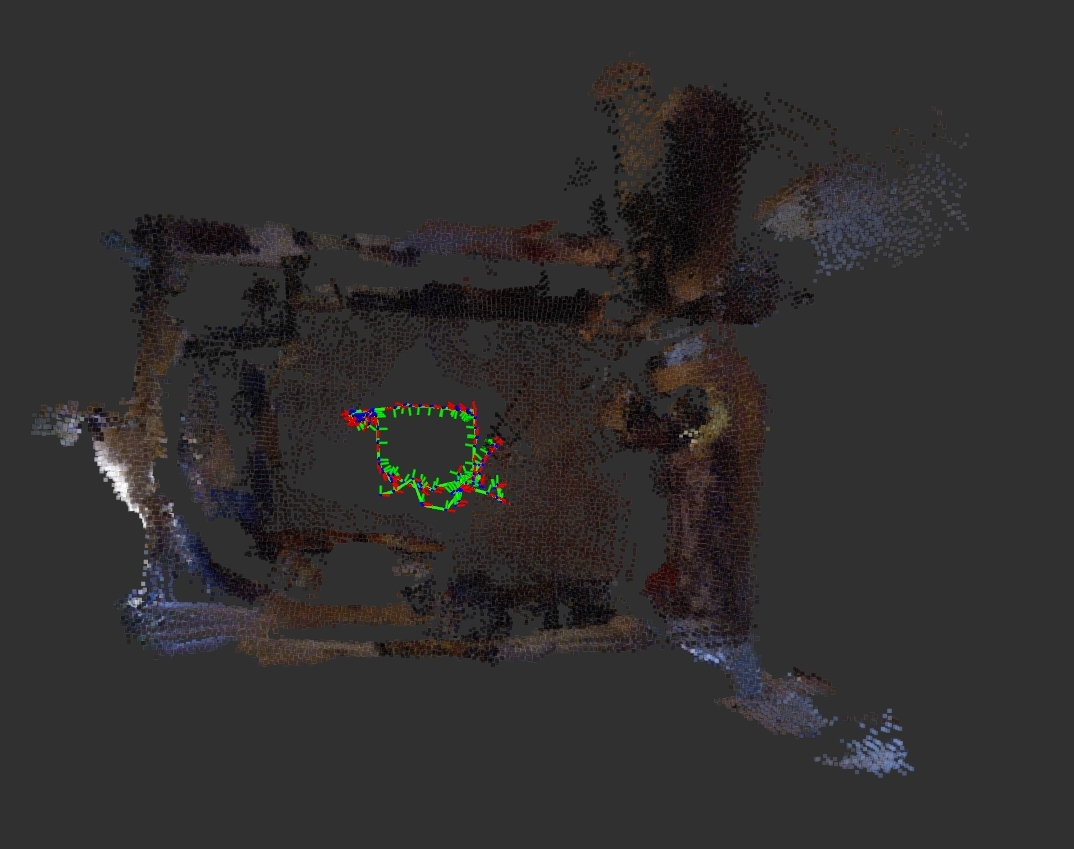
\includegraphics[width=.415\textwidth]{images/slam/bag1_rtabmap_LC}
    \caption{Mapa creado ántes y después del \textit{Loop Closure}}
\end{figure}

El mapa obtenido, será un mapa denso el cual posee toda la información posible del entorno, cómo se muestra a continuación:
\begin{figure}[h!]
    \centering
    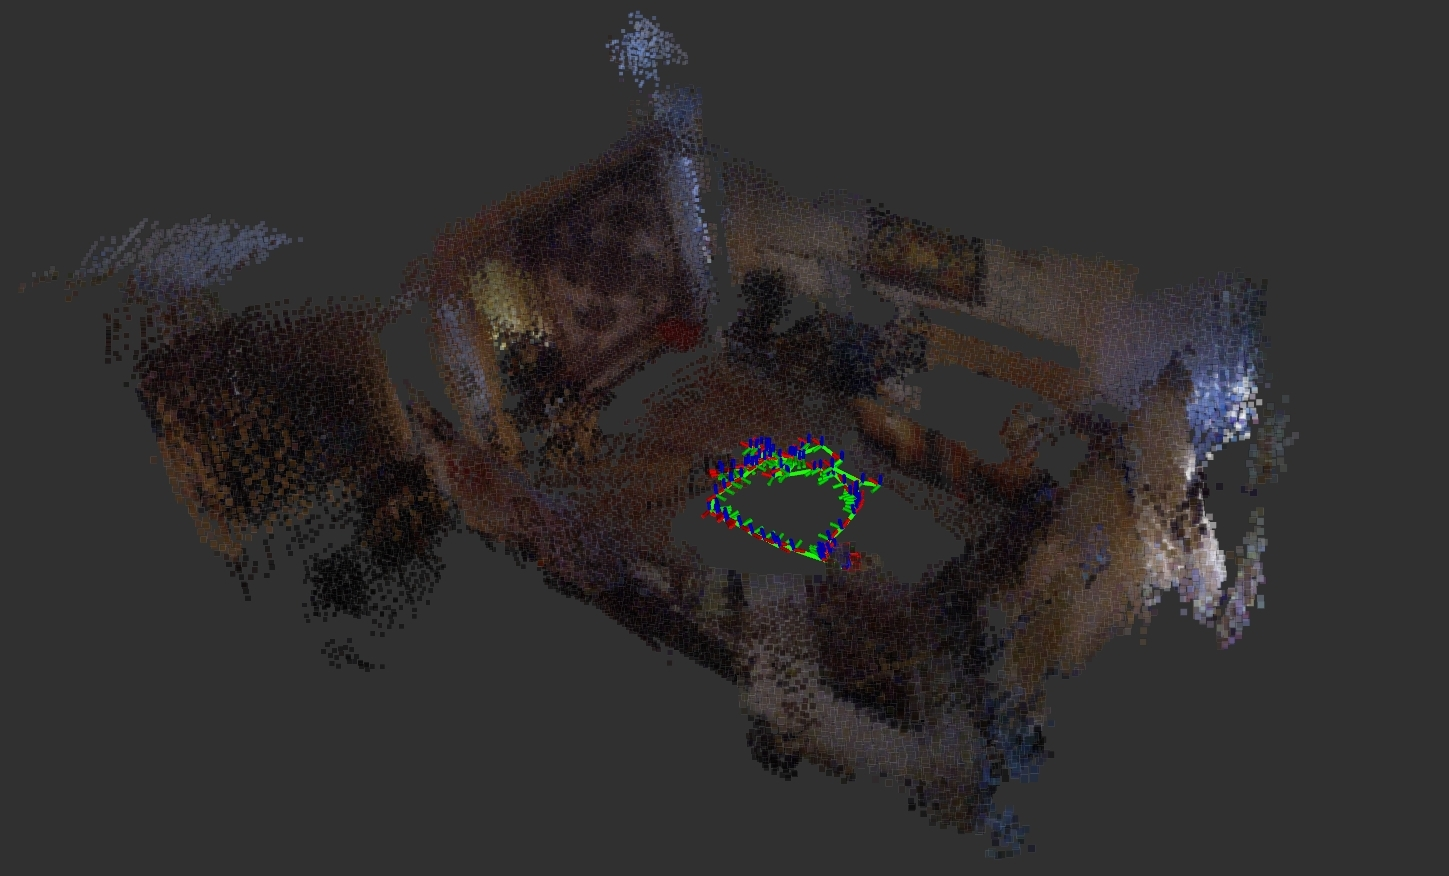
\includegraphics[width=.9\textwidth]{images/slam/bag1_rtabmapbonito}
    \caption{Mapa obtenido con RTAB-Map}
\end{figure}

Gracias a la realización de dicho mapa, se ha optado por medir la tela grande de la pared y el cuadro sobre el sillón naranja tanto en el mapa cómo la distancia real, para comprobar
el error que posee ésta técnica.

\begin{center}
\begin{tabular}{ c | c | c | c }
     & Ancho en el mapa creado & Ancho real & Error de RTAB-Map\\
     \hline
     Tela de la pared & 1.72 m & 1.8 m & 0.08 m\\
     Cuadro sobre sillón & 1.07 m & 1.13m & 0.05m\\
\end{tabular}
\end{center}

Se observa cómo, el error de ésta técnica de SLAM frente a las medidas reales es casi un orden de magnitud menor, algo que se considera asumible.

\subsubsection{OctoMap}
Gracias a \textit{Octomap} se ha obtenido el mapa de ocupación probabilístico del entorno. Se mostrará, al igual que antes, el mapa ántes y después del loop closure, ya que es lo
destacable de ésta técnica de SLAM.
\begin{figure}[h!]
    \centering
    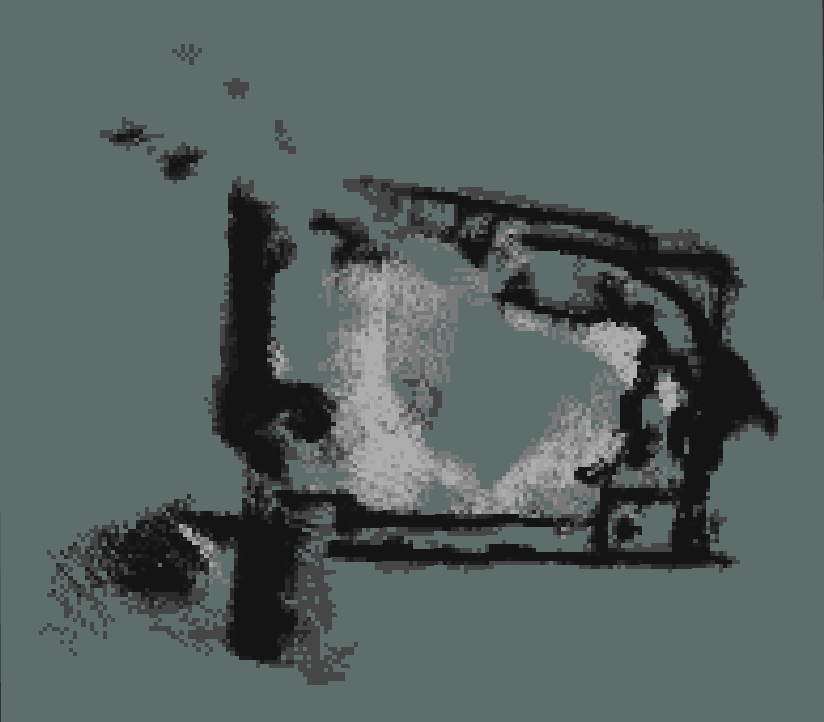
\includegraphics[width=.4\textwidth]{images/slam/bag1_occupGrid_noLC}
    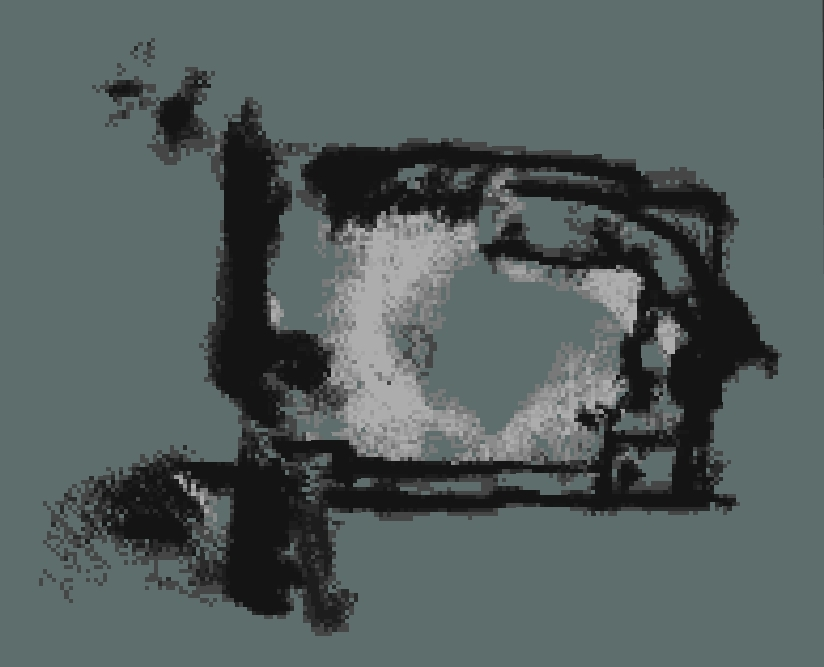
\includegraphics[width=.435\textwidth]{images/slam/bag1_occupGrid_LC}
    \caption{Mapa de ocupación ántesy despues del \textit{Loop Closure}}
\end{figure}

Además, \textit{Octomap} nos proporciona el mapa de ocupación 3D, cómo el mostrado a continuación:
\begin{figure}[h!]
    \centering
    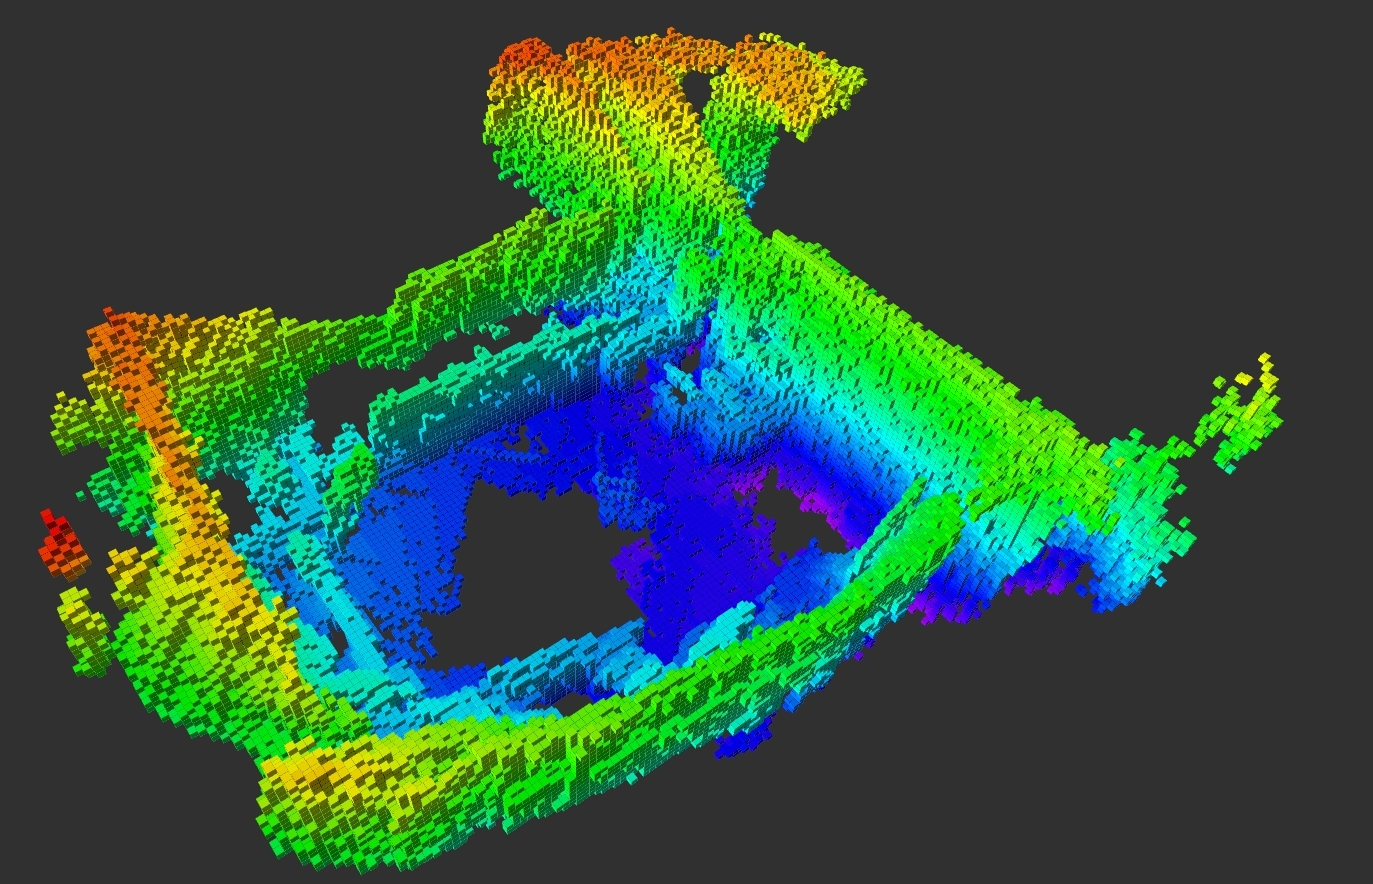
\includegraphics[width=.9\textwidth]{images/slam/bag1_octomap_LC}
    \caption{Mapa obtenido con RTAB-Map y empleando el framework \textit{Octomap}}
\end{figure}

\subsubsection{ORB-SLAM2 RGB-D}
En el caso del ORB-SLAM2, con este dataset los resultados han sido peores, debido a que en cierto momento, los cambios de iluminosidad procedentes del balcón de la casa, hacen que se
se pierda dentro del mapa creado. A continuación se muestra el frame anterior a la pérdida de la localización dentro del mapa. Los colores representan la altura en el eje Z.
\begin{figure}[h!]
    \centering
    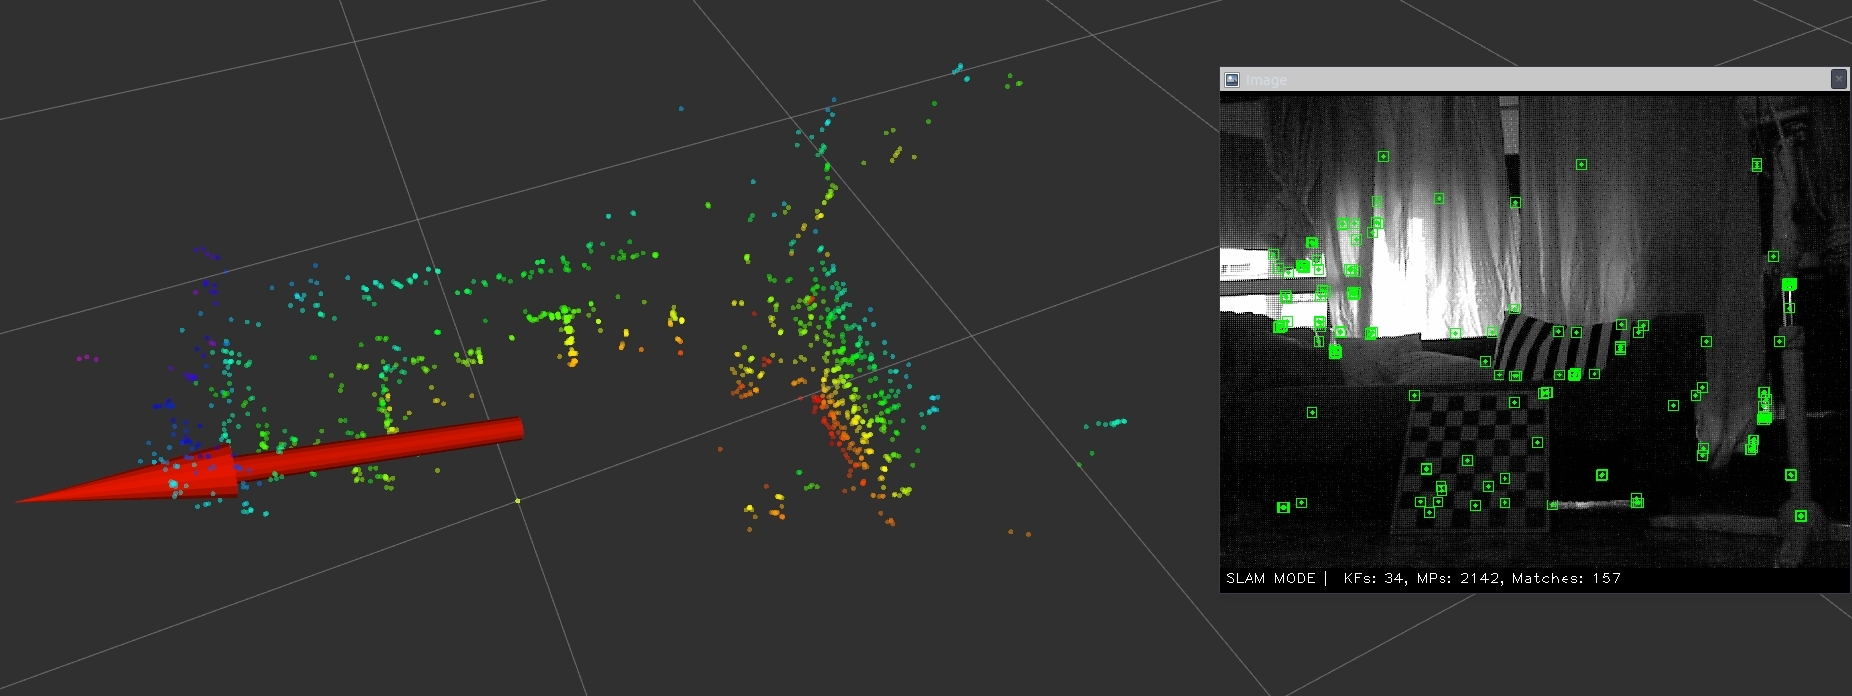
\includegraphics[width=.9\textwidth]{images/slam/bag1_orb_beforeLOSE}
    \caption{Momento anterior a la pérdida del robot en el primer dataset}
\end{figure}

Sin embargo, se observa cómo, cuándo vuelve a ver el inicio del mapa, dónde tomó un número elevado de features, se relocalizará, cómo se muestra a continuación:
\begin{figure}[h!]
    \centering
    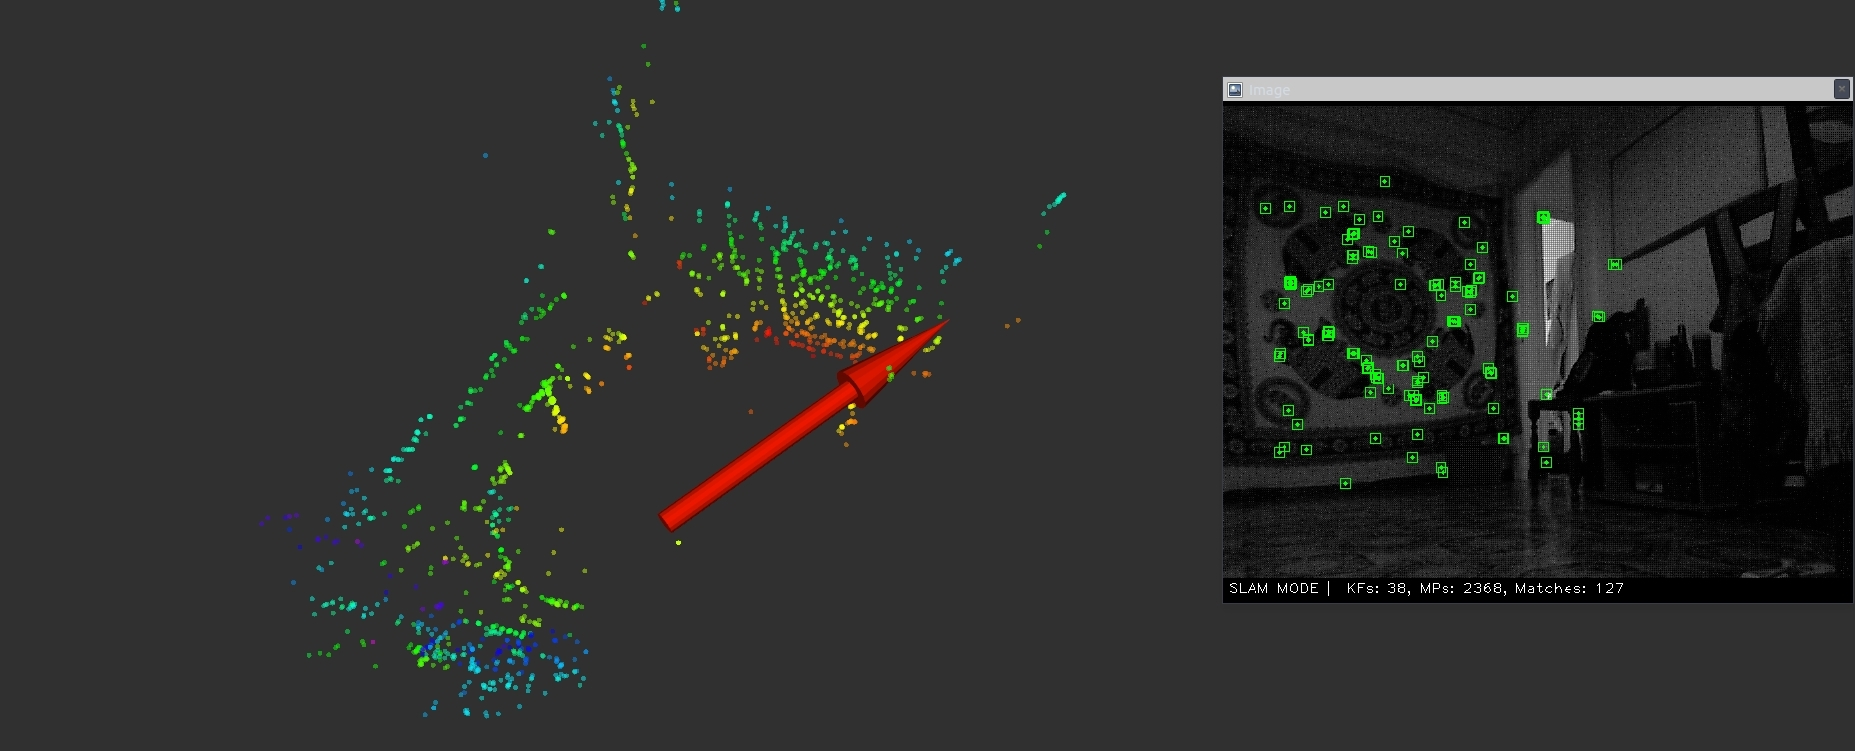
\includegraphics[width=.9\textwidth]{images/slam/bag1_orb_relocal}
    \caption{Relocalización del robot en el primer dataset}
\end{figure}

Debido a que el mapa no se ha llegado a completar se ha obtado por no realizar una comparativa de las medidas en éste caso.

\newpage

\subsection{Análisis de resultados con el segundo \textit{rosbag}}
En éste segundo dataset, el escenario será más parecido a un escenario experimental debido a que se han colocado objetos por el salón de tal modo que en todo el mapa se
obtengan una cantidad elevada de features.

\subsubsection{RTAB-Map y local path}
Al igual que anteriormente, se destacará el loop closure detectado por el mapa. Se observa cómo, ántes de dicho momento, las imágenes de la tela de la pared aparecen superpuestas,
y sin embargo, posteriormente, se observa cómo ha detectado que ya conocia ese setpoint y cerró el bucle:
\begin{figure}[h!]
    \centering
    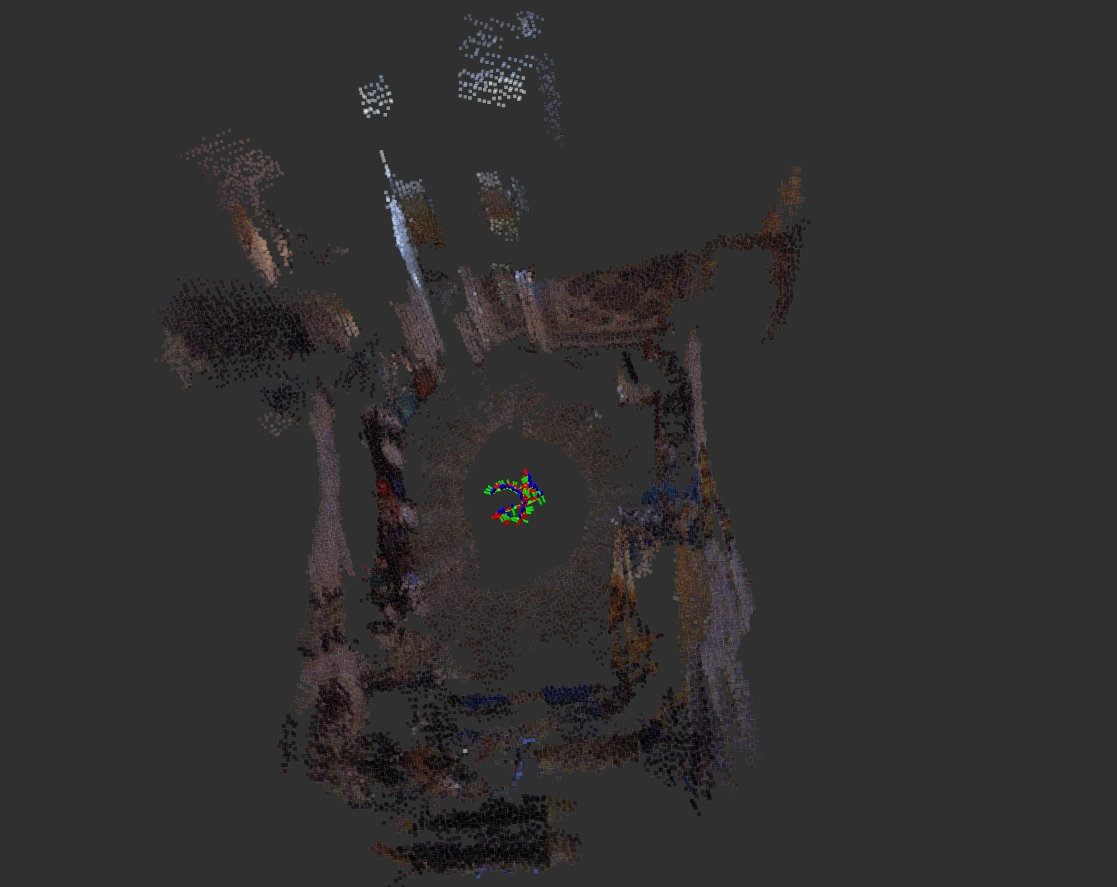
\includegraphics[width=.4\textwidth]{images/slam/bag3_rtabmap_noLC}
    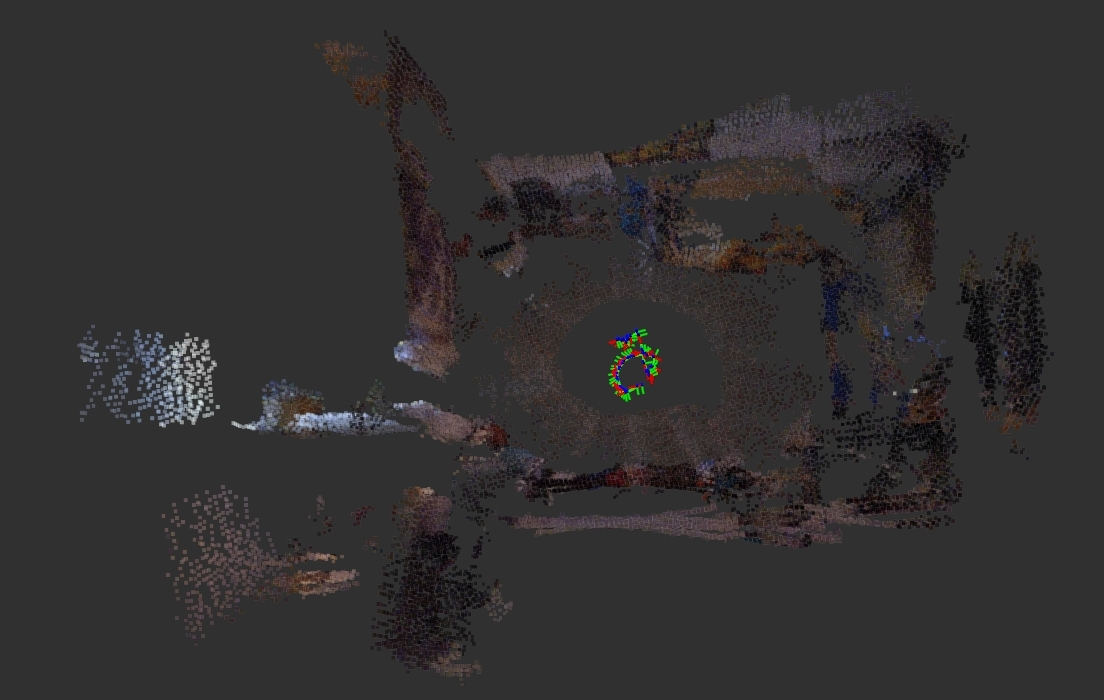
\includegraphics[width=.51\textwidth]{images/slam/bag3_rtabmap_LC}
    \caption{Mapa creado ántes y después del \textit{Loop Closure} con el segundo dataset}
\end{figure}

El mapa obtenido, será un mapa denso el cual posee toda la información posible del entorno, cómo se muestra a continuación:

\begin{figure}[h!]
    \centering
    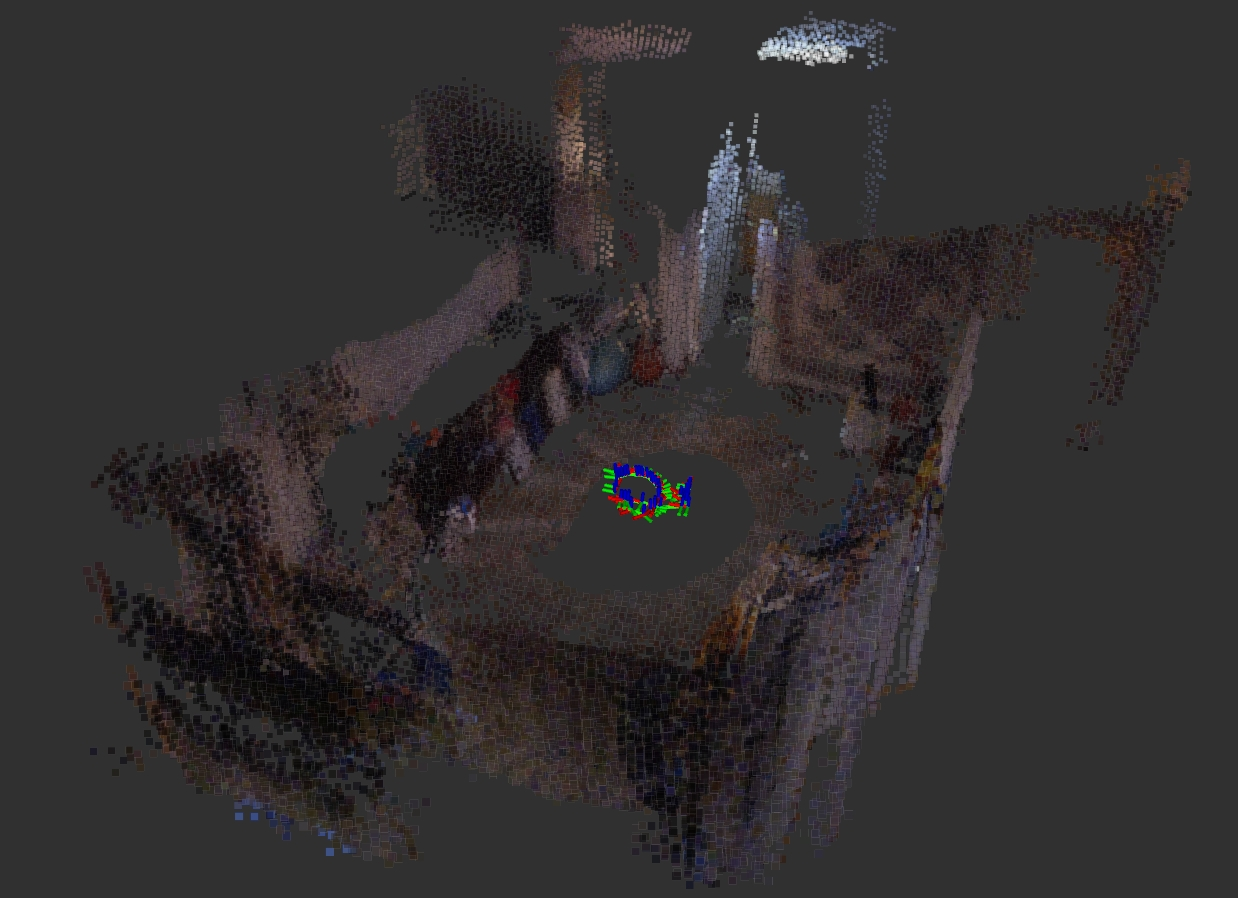
\includegraphics[width=.7\textwidth]{images/slam/bag3_rtabmapbonito}
    \caption{Mapa obtenido con RTAB-Map empleando el segundo dataset}
\end{figure}
    
\newpage
    \subsubsection{OctoMap}
Gracias a \textit{Octomap} se ha obtenido el mapa de ocupación probabilístico del entorno. Se mostrará, al igual que antes, el mapa ántes y despues del loop closure, ya que es lo
destacable de ésta técnica de SLAM.
\begin{figure}[h!]
    \centering
    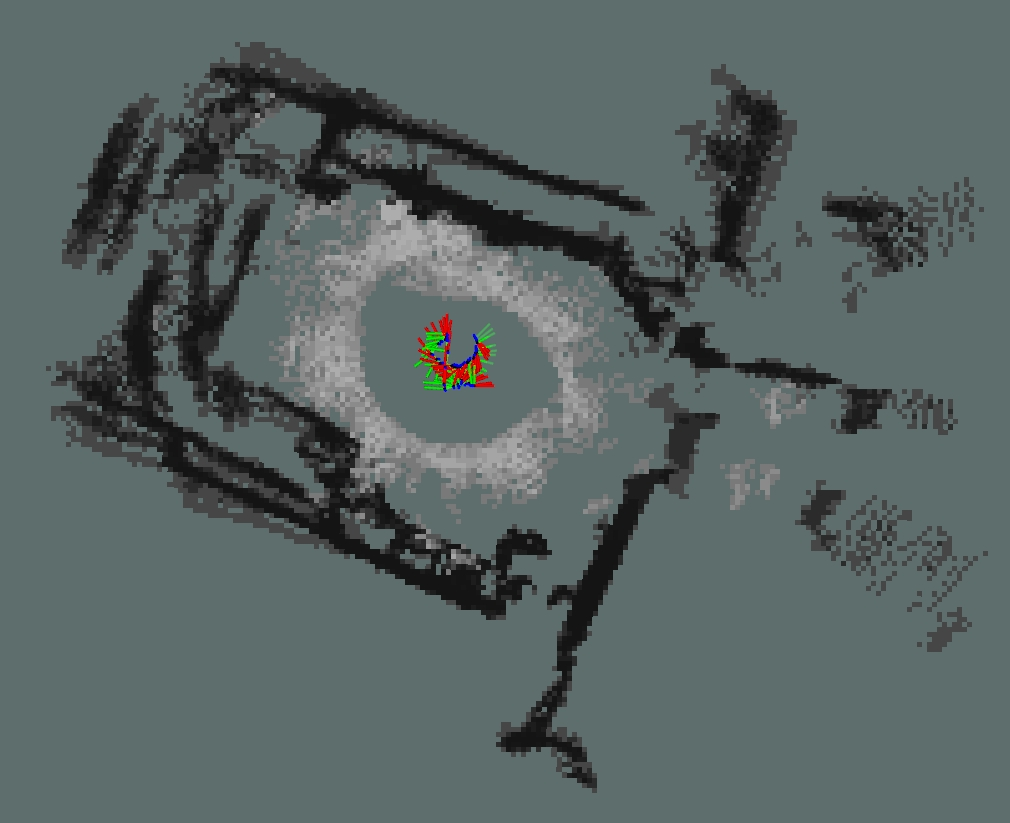
\includegraphics[width=.4\textwidth]{images/slam/bag3_occupGrid_noLC}
    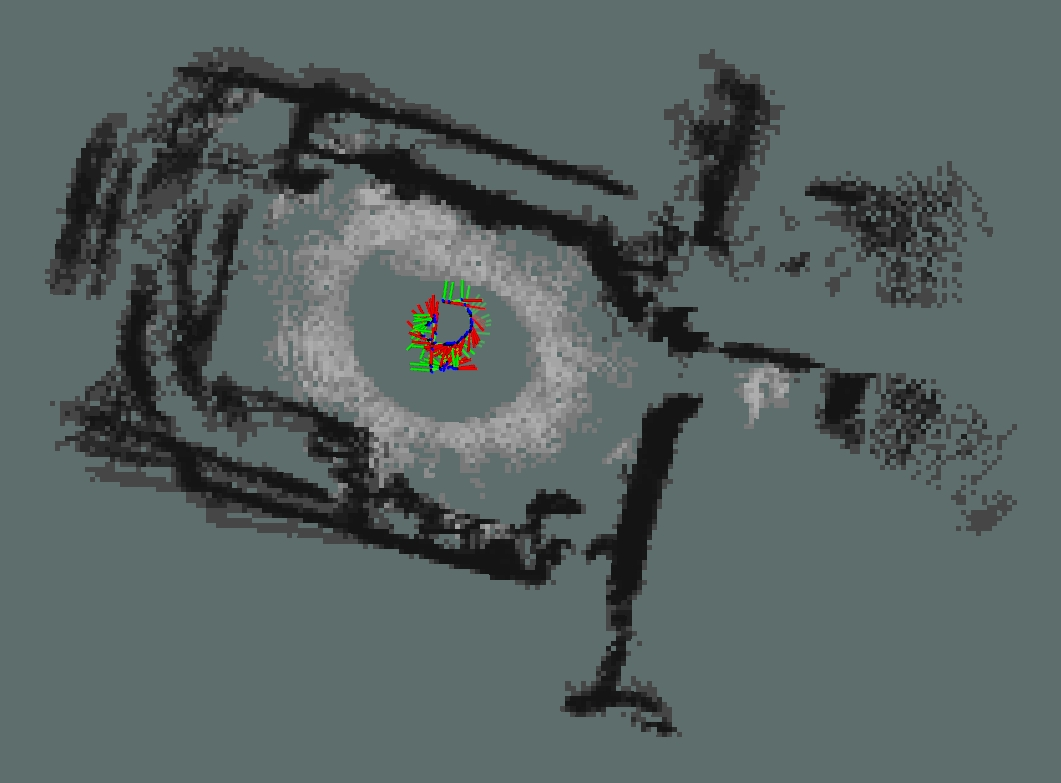
\includegraphics[width=.435\textwidth]{images/slam/bag3_occupGrid_LC}
    \caption{Mapa de ocupación ántes y despues del \textit{Loop Closure}}
\end{figure}

Además, \textit{Octomap} nos proporciona el mapa de ocupación 3D, cómo el mostrado a continuación:
\begin{figure}[h!]
    \centering
    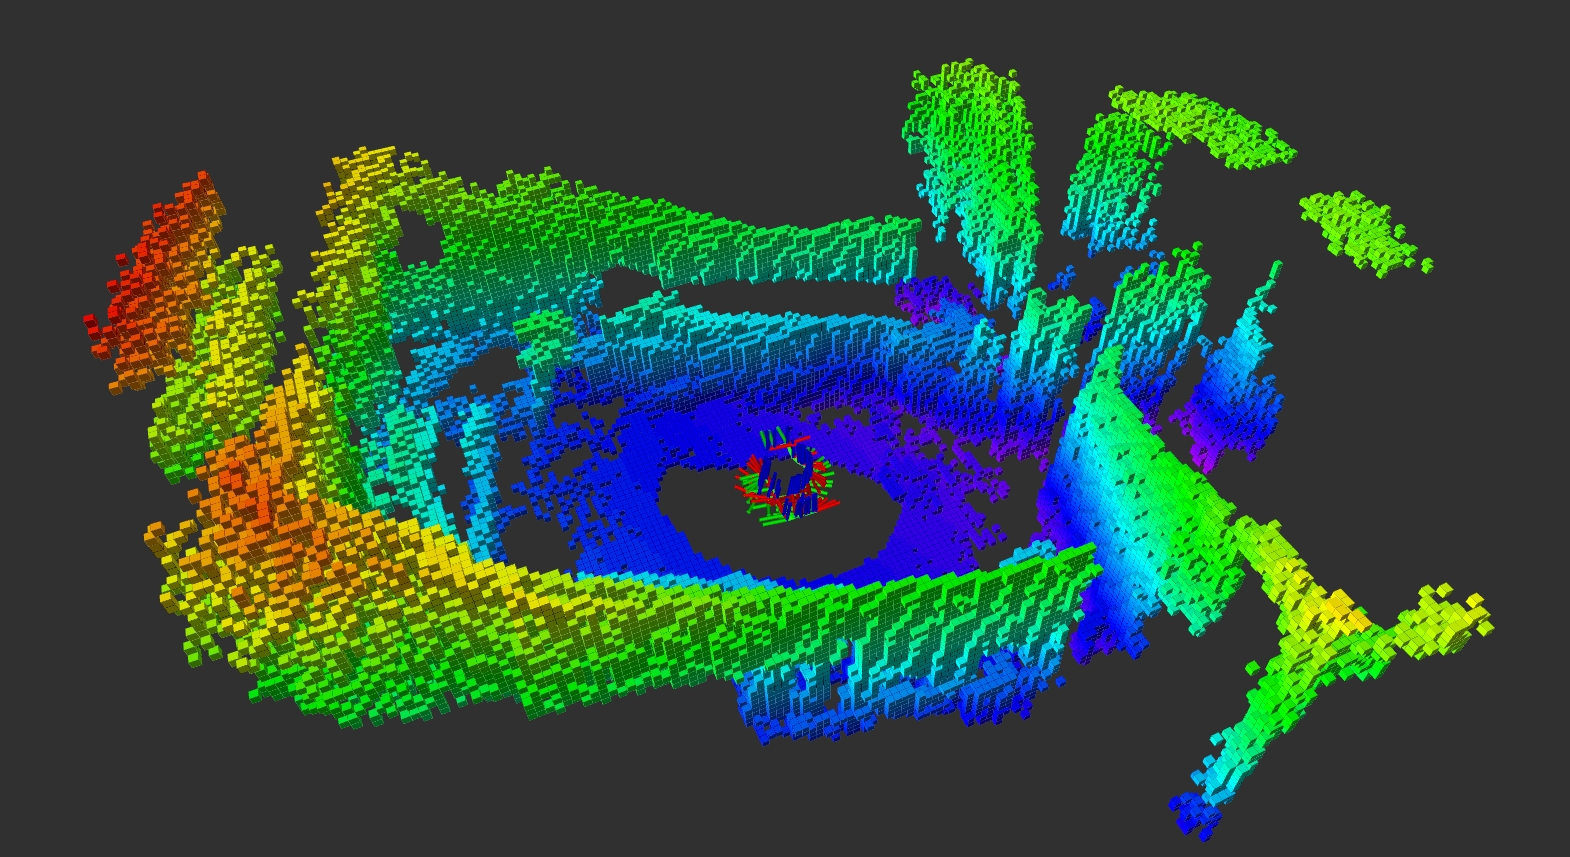
\includegraphics[width=.9\textwidth]{images/slam/bag3_octomap_LC}
    \caption{Mapa obtenido con RTAB-Map y empleando el framework \textit{Octomap}}
\end{figure}

\newpage
\subsubsection{ORB-SLAM2 RGB-D}
En éste segundo set de datos, se evitó el cambio de iluminación en el punto dónde ántes se perdio, de tal modo que en éste caso no pase y, efectivamente, cómo se mostrará a continuación,
en ese punto no se perdió:
\begin{figure}[h!]
    \centering
    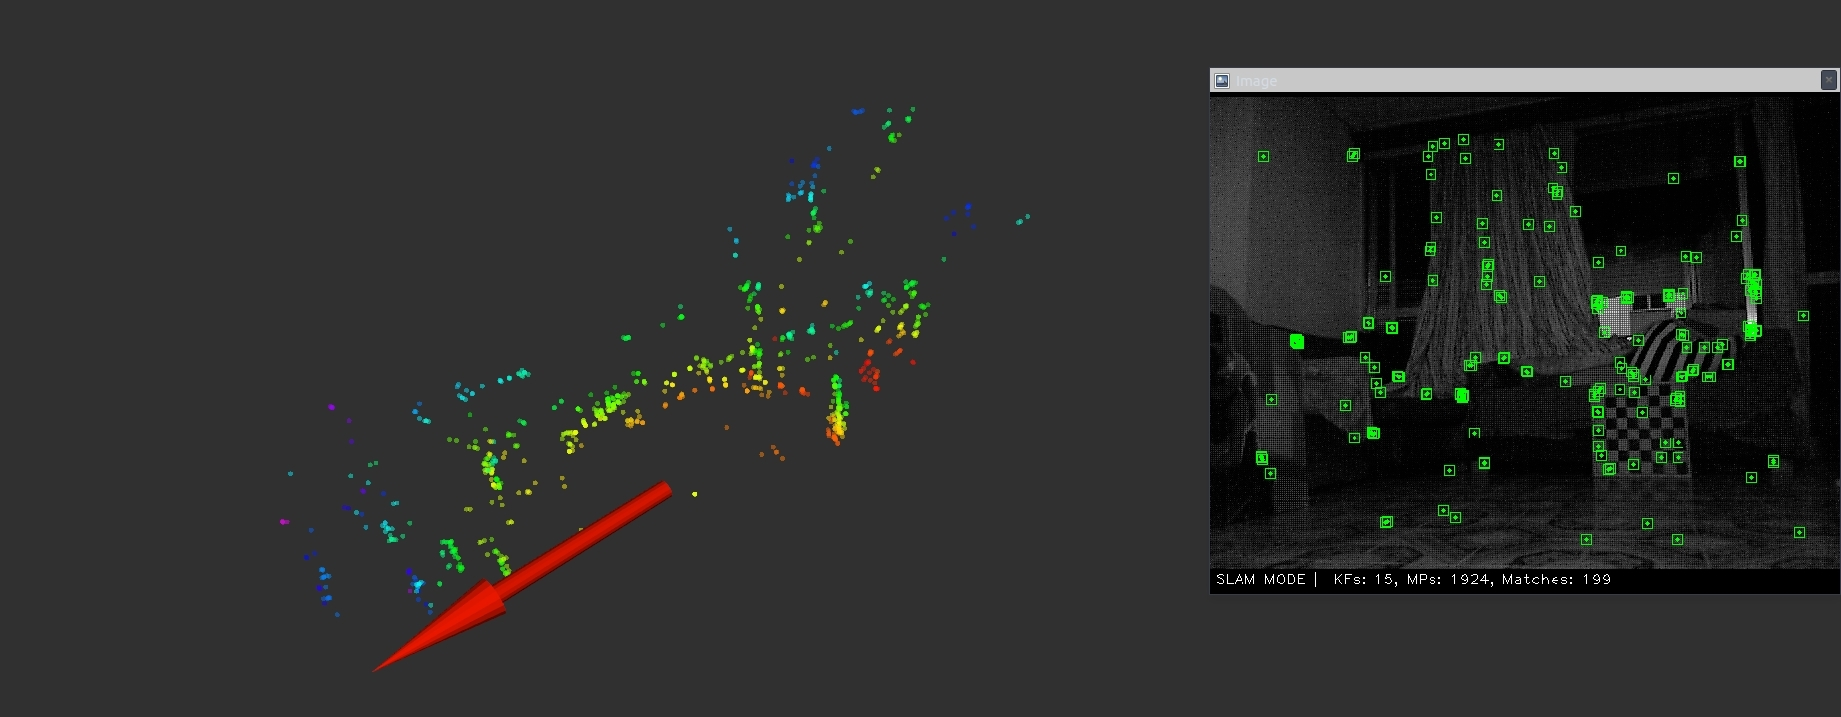
\includegraphics[width=.9\textwidth]{images/slam/bag3_orb_avoidLOSE}
    \caption{Modificación del entorno para evitar la perdida de ORB}
\end{figure}

Por tanto, en éste caso sí se ha logrado obtener un mapa disperso del entorno:
\begin{figure}[h!]
    \centering
    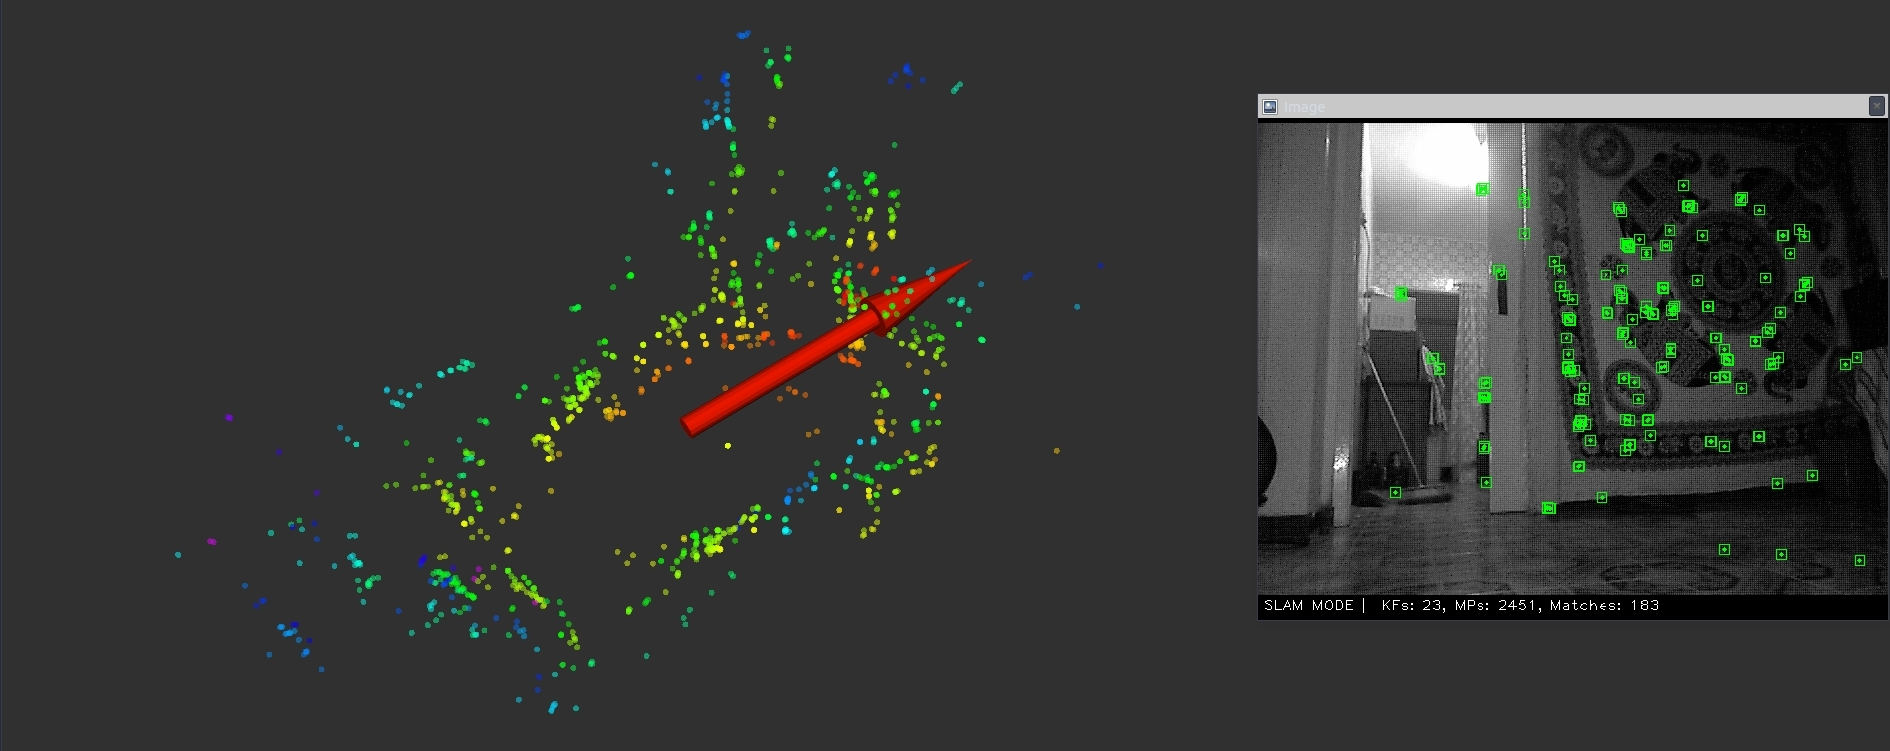
\includegraphics[width=.9\textwidth]{images/slam/bag3_orb_map}
    \caption{Mapa del entorno empleando ORB-SLAM2}
\end{figure}

Se observa cómo, el mapa obtenido empleando ésta técnica se basa mayoritariamente en la detección de los features del entorno. En comparativa con RTAB-Map, ésta técnica podría parecer
mucho peor, sin embargo, bajo un ordenador de altas prestaciones los resultados para robótica sin muy destacables ya el mapa disperso es completamente funcional para poder relocalizarse
y, de ese modo, conocer la posición del robot móvil que esté implementando el SLAM en ese momento.
\newpage
\subsection{Resultados obtenidos de ORB-SLAM2 Monocular}
Debido a la compleja inicialización que conlleva emplear ésta técnica monocular, no ha sido posible evaluar su funcionamiento con los bags generados, ya que no se logró que se
inicializase. Sin embargo, para comprobar su funcionamiento, se ha optado por mover la cámara \textit{Hand-handle}, de tal modo que se asegure la inicialización del SLAM. \\
El gran punto a favor que posee el empleo de SLAM monocular es que no es sensible a la luz, de tal modo que funciona correctamente en exteriores. \\
Por ello, la prueba realiza es en el mismo salón, pero saliendo al balcón y grabando al exterior. \\

Para inicializar el SLAM, ha sido necesario asegurarse que se tomaban y se lograban tracker las \textit{features} de la tela de la pared. A continuación, se mostrará una imagen
del mapa grabado durante bastante tiempo, asegurandose de que se tomaban los suficientes puntos característicos y, se intentó realizar una prueba de cómo estima la altura del piso, 
saliendo al balcón y haciendo que la cámara apuntase al suelo. Es por ello que el mapa tiene la siguiente forma:

\begin{figure}[h!]
    \centering
    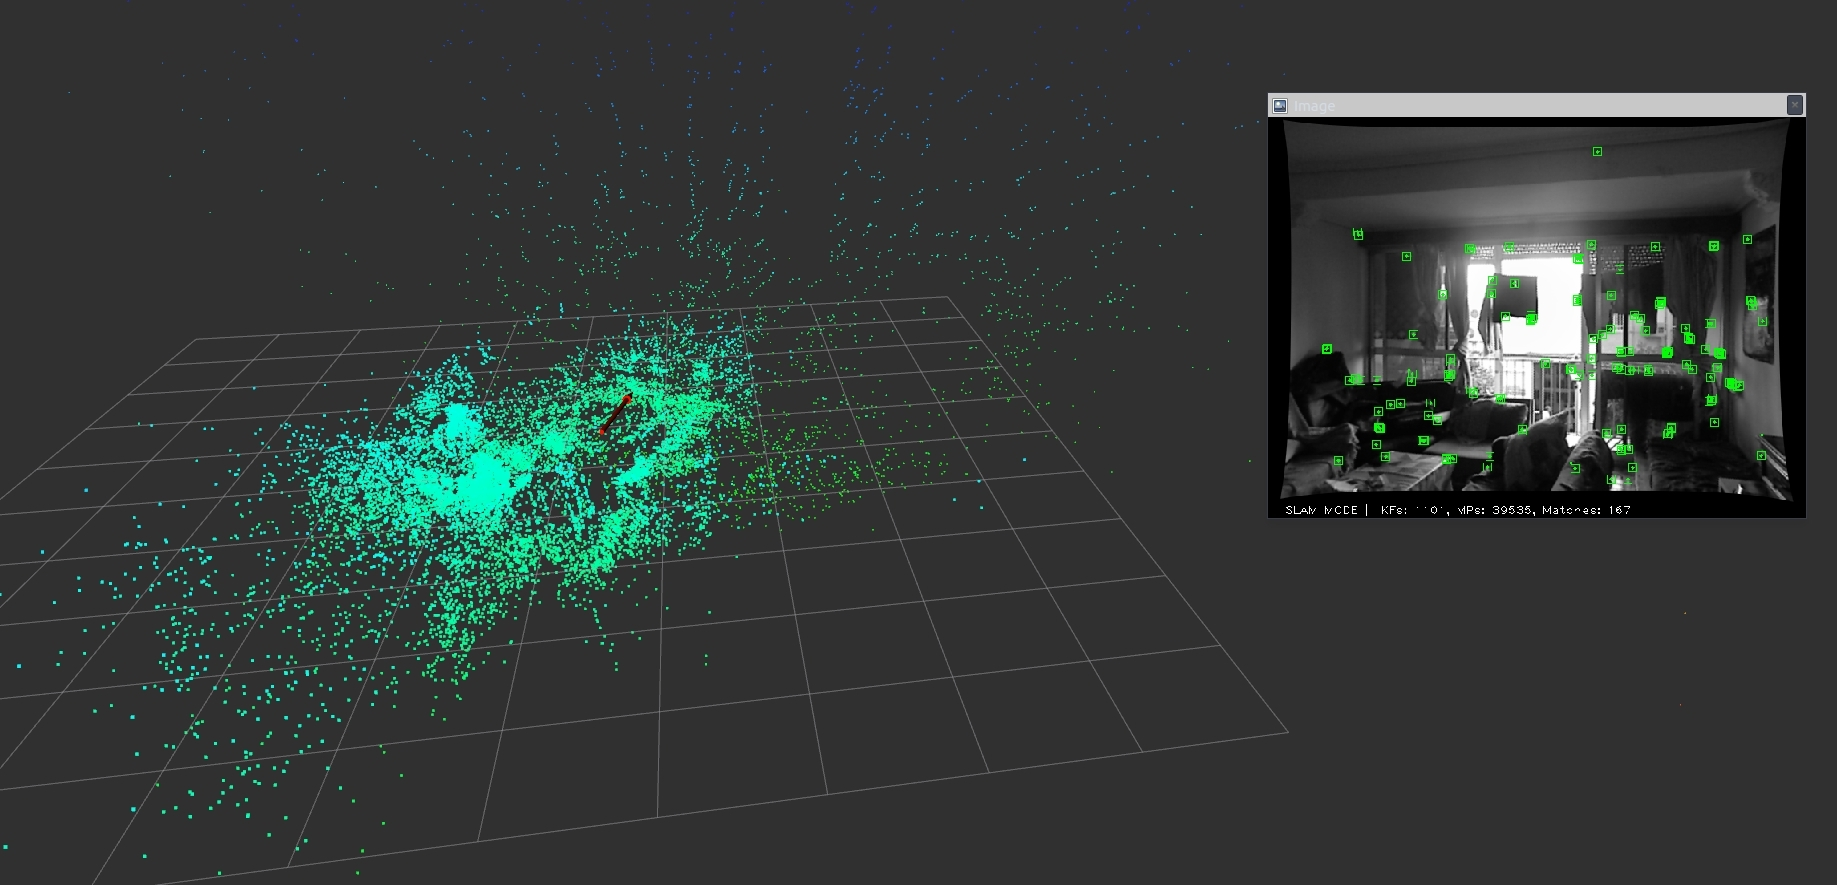
\includegraphics[width=.9\textwidth]{images/slam/mono}
    \caption{Mapa del entorno empleando ORB-SLAM2 Monocular Hand-Handle}
\end{figure}

Se observa cómo ésta técnica es insensible a los cambios de luminosidad en la imagen anterior y los puntos alejados que ha tomado son features tomadas de los edificios de enfrente de la
casa.
